\documentclass[../../Main/Appunti Fisica.tex]{subfiles}
\begin{document}
Uno strumento utile per lo studio dei gas, è il modello della teoria cinetica.\\
Questa si basa sulle seguenti ipotesi
\begin{enumerate}
    \item Il numero di molecole presenti nel gas è elevato, e la distanza tra ciascuna di esse, se paragonata alle dimensioni, è grande.
    \item Ciascuna particella, se considerata a solo, segue le leggi di Newton; nel complessivo invece il moto è casuale.
    \item Le molecole interagiscono mediante forze a corto raggio, forze le quali si esercitano in urti elastici.
    \item Il gas analizzato è una sostanza pura.
\end{enumerate}
%
Si consideri ora la figura di seguito riportata.
\begin{figure}[!h]
    \centering
    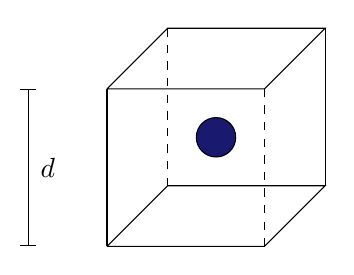
\begin{tikzpicture}[scale = 1, every node/.style={scale=1}]

        % Cubic container
        \draw (0, 0, 0) -- (0, 0, -2) -- (2, 0, -2) -- (2, 0, 0) -- (0, 0, 0);
        \draw (0, -2, 0) -- (0, -2, -2) -- (2, -2, -2) -- (2, -2, 0) -- (0, -2, 0);
        \draw (0, 0, 0) -- (0, -2, 0);
        \draw [dashed] (0, 0, -2) -- (0, -2, -2);
        \draw (2, 0, -2) -- (2, -2, -2);
        \draw [dashed] (2, 0, 0) -- (2, -2, 0);

        \draw [|-|] (-1, 0, 0) -- (-1, -2, 0);
        \node (anchor = east) at (-0.75, -1, 0) {\(d\)};

        % Single particle
        \draw [fill = MidnightBlue] (1, -1, -1) circle (0.25);

    \end{tikzpicture}
    \caption{Gas contenuto in contenitore cubico.}
    \label{fig:10}
\end{figure}

Si supponga che la sfera in blu in Figura \ref{fig:10}, rappresenti del gas a volume \(V\) costituito da \(N\) molecole.
\\ \\
Supponendo che ciascuna delle \(N\) molecole abbia massa \(m_{0}\) e velocità lungo l'asse \textit{x} \(\vb{v_{xi}}\),
se considerata la quantità di moto \(\vb{p}\), poiché la massa della parete è molto maggiore di \(m_{0}\),
segue che \(\vb{p_{xi}} = m_{0} \vb{v_{xi}}\) antecedentemente l'urto e \(- m_{0} \vb{v_{xi}}\) successivamente.
\\
Ma allora segue
\[
    \Delta \vb{p} = -m_{0}\vb{v_{xi}} - (m_{0}\vb{v_{xi}}) = - 2 m_{0}\vb{v_{xi}}
\]
%
Poiché ciascuna molecola è soggetta alle leggi di Newton, segue dal teorema dell'impulso
\[
    \va{F_{m}} {\Delta t_{u}} = \Delta \vb{p_{xi}} = - 2 m_{0}\vb{v_{xi}}
\]
ove \(\va{F_{m}}\) è la forza esercitata dalla parete sulla molecola, \(\Delta t_{u}\) la durata dell'urto.

Segue che affinché la singola molecola urti nuovamente una stessa parete, è necessario che la stessa percorra una distanza \(2d\), da cui
\[
    \Delta t = \frac{2d}{\vb{v_{xi}}}
\]
%
Sebbene la forza che causa una variazione della quantità di moto sia presente solo durante l'urto, è possibile stabilire una forza media \(\mv{F_{i}}\) nell'intervallo tra andata e ritorno,
segue
\[
    \va{F_{i}} \Delta t = - 2 m_{0}\vb{v_{xi}}
\]
da cui, se applicata la terza legge di Newton, segue che sulla parete si esercita una forza
\[
    \mv{F} = - \mv{F_{i}} = \frac{m_{0}\vb{v_{xi}}^{2}}{d}
\]
%
La forza totale \(\mv{F}\) è allora data da
\[\begin{aligned}
        \mv{F} & = \sum\limits_{i = 1}^{N}{\frac{m_{0}\vb{v_{xi}}}{d}}  \\
               & = \frac{m_{0}}{d} \sum\limits_{i = 1}^{N}{\vb{v_{xi}}}
    \end{aligned}\]
ma da cio segue
\[
    \mv{v_{xi}} = \frac{\sum\limits_{i = 1}^{N}{v_{xi}}}{N}
\]
%
Si può quindi scrivere \(\mv{F}\) come
\[
    \mv{F} = \frac{m_{0}}{d} N \mv{v_{xi}^{2}}
\]
%
Si consideri una singola molecola, questa avrà velocità \(\va{v_{i}^{2}} = \vb{v_{xi}^{2}} + \vb{v_{yi}}^{2} + \vb{v_{zi}^{2}}\),
segue che \(\mv{v} = \vb{v_{x}^{2}} + \vb{v_{y}}^{2} + \vb{v_{z}^{2}}\).
Poiché il moto è casuale segue \(\vb{v_{xi}}^{2} = \vb{v_{yi}}^{2} = \vb{v_{zi}}^{2}\). \\
Cioè
\[
    \mv{v_{i}} = 3 \mv{v_{xi}}
\]
%
allora
\[
    \mv{F} = \frac{1}{3} N \frac{m_{0} \mv{v}^{2}}{d}
\]
%
Calcolando ora la pressione \(\vb{P}\), segue
\[\begin{aligned}
    \vb{P} = \frac{\mv{F}}{A} &= \frac{1}{3} N \frac{m_{0} \mv{v}^{2}}{d^{3}} \\
    &= \frac{2}{3} \frac{N}{V} \frac{1}{2} m_{0} \mv{v^{2}}
\end{aligned}\]

\subsubsection{Interpretazione molecolare della temperatura.}
Si considerino le due equazioni per il calcolo di \(PV\).
\[
\vb{P}V  = \frac{2}{3} \frac{N}{V} \frac{1}{2} m_{0} \mv{v^{2}} = N K_{B} T
\]
%
Segue
\[
    T = \frac{2}{3 K_{B}} \left( \frac{1}{2}m_{0} \mv{v^{2}} \right)
\]
%
Poiché \(\vb{v_{x}^{2}} = \frac{1}{3} \mv{v^{2}}\), e cosi analogamente \(\vb{v_{y}^{2}}, \vb{v_{z}^{2}}\), segue
\[
    \frac{1}{2} m_{0} \mv{v_{2}^{2}} = \frac{1}{2} K_{B} T
\]
%
Quanto detto è generalizzato nel \textit{teorema dell'equipartizione dell'energia}.
\begin{Theorem*}[dell'equipartizione dell'energia]
    Ogni grado di libertà dà contributo \(\frac{1}{2} K_{B} T\) all'energia totale del sistema.
\end{Theorem*}
\end{document}
\clearpage